\section{Simulazioni modello di Ising 2D}

%-----------------------------------------%
%				Prima slide				  %
%	   Caratterizzazione metropolis   	  %
%-----------------------------------------%
\begin{frame}
    \frametitle{Caratterizzazione con metropolis}
    \framesubtitle{}

    \begin{columns}
        \begin{column}{0.33\textwidth}
            \begin{block}{Termalizzazione}

                \begin{itemize}[itemsep=0.5em, label=$\diamond$]
                    \item $t_{ter}$ maggiori per $T \simeq T_c$
                    \item $t_{ter}^{max}\,\simeq\,500$ sweeps
                \end{itemize}

                \vspace{0.5cm}

                \centering
                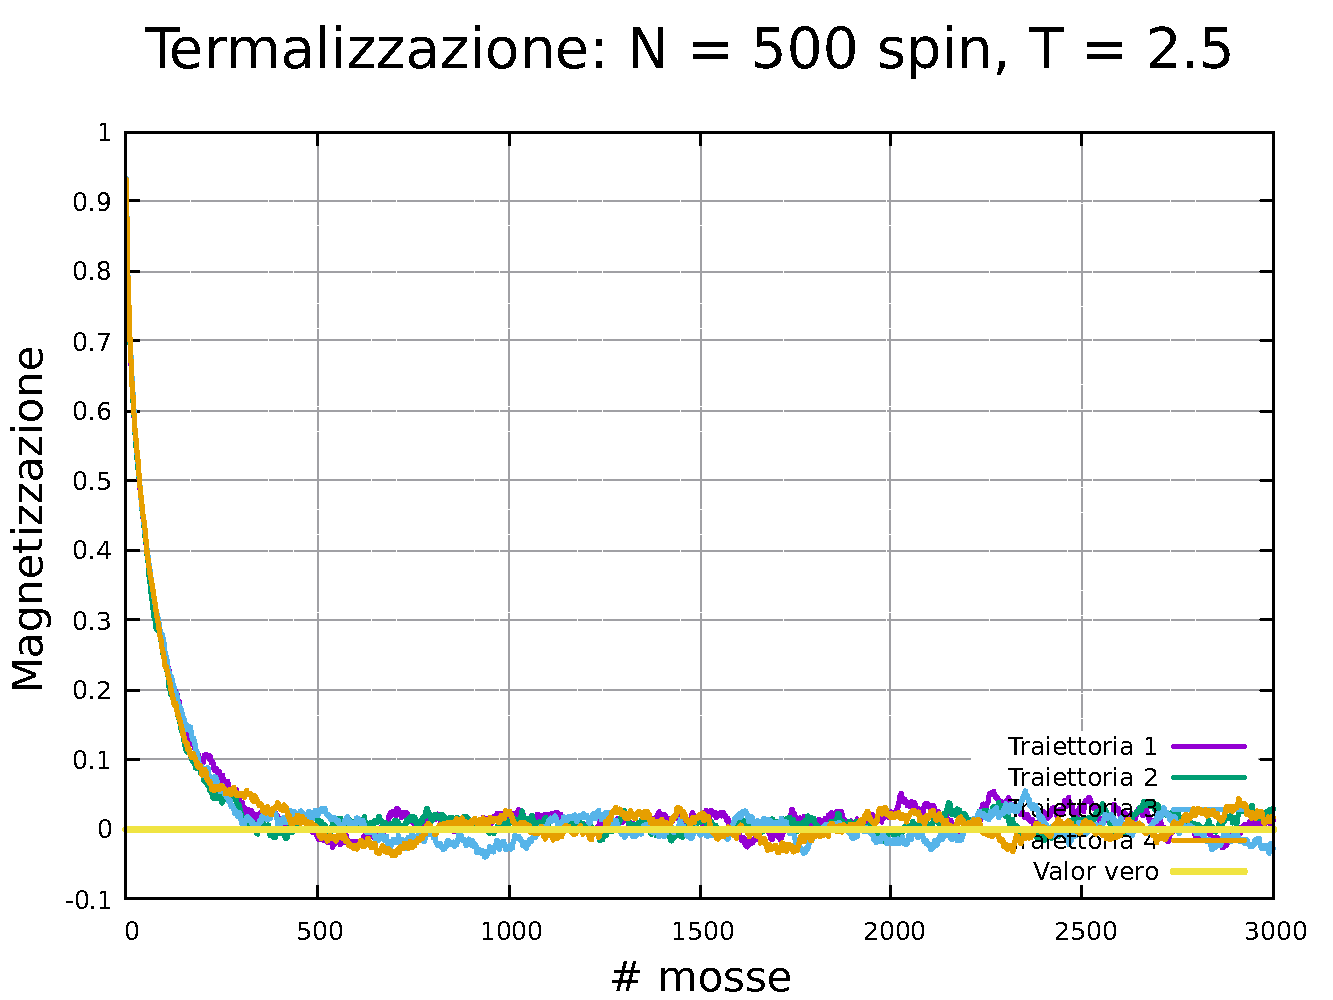
\includegraphics[width=\textwidth]{Immagini/simIsing2D/term_500_2.5.pdf}
            
            \end{block}
        \end{column}
    
        \begin{column}{0.33\textwidth}
            \begin{block}{Auto-correlazione}

                \begin{itemize}[itemsep=0.5em, label=$\diamond$]
                    \item $t_{c}$ maggiori per $T \simeq T_c$
                    \item $t_{c}^{max}\,\simeq\,400$ sweeps
                \end{itemize}

                \vspace{0.5cm}

                \centering
                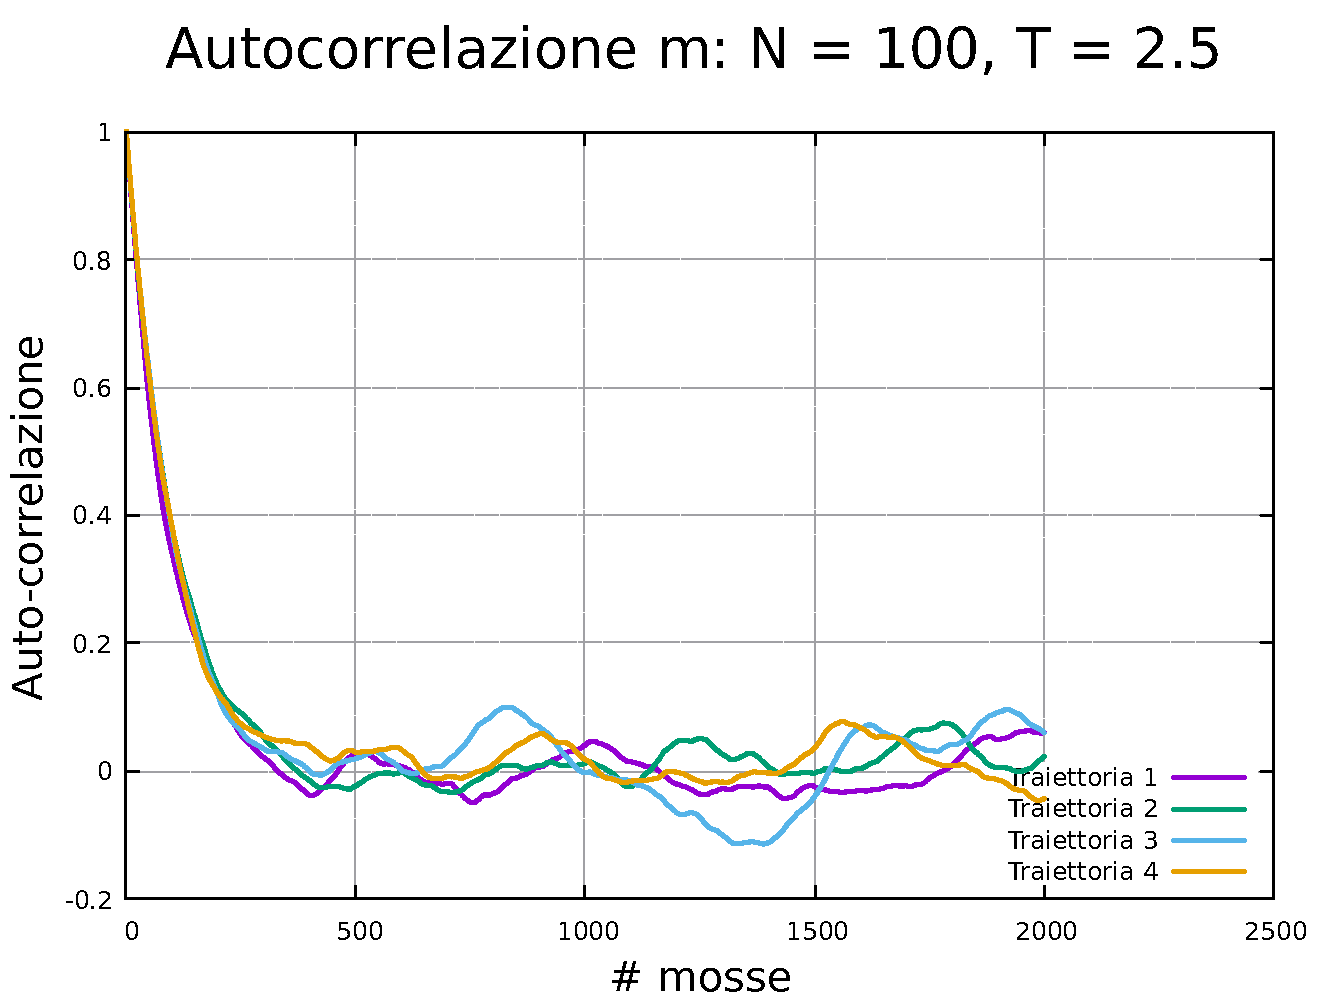
\includegraphics[width=\textwidth]{Immagini/simIsing2D/auto_100_2.5.pdf}
            
            \end{block}
        \end{column}

        \begin{column}{0.33\textwidth}
            \begin{block}{Blocchi}

                \begin{itemize}[itemsep=0.5em, label=$\diamond$]
                    \item $l_{blk}$ maggiori per $T \simeq T_c$
                    \item $l_{blk}^{max}\,\simeq\,1000$ sweeps
                \end{itemize}

                \vspace{0.5cm}

                \centering
                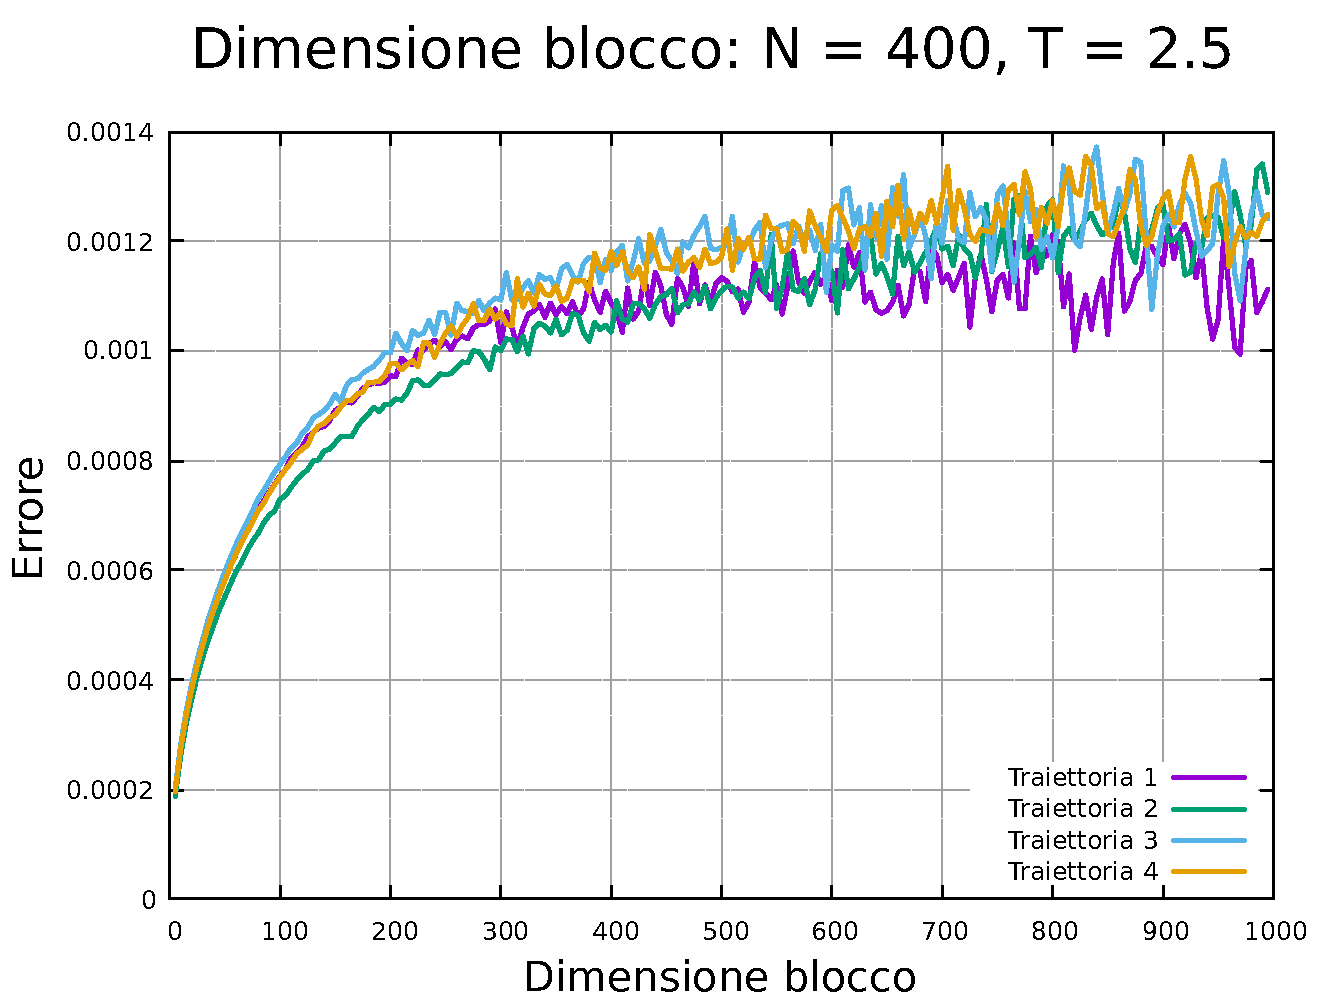
\includegraphics[width=\textwidth]{Immagini/simIsing2D/err_400_2.5.pdf}

            \end{block}        
        \end{column}
    \end{columns}
\end{frame}



%-----------------------------------------%
%		        Seconda slide	    	  %
%	      Caratterizzazione wolff   	  %
%-----------------------------------------%
\begin{frame}
    \frametitle{Caratterizzazione con Wolff}
    \framesubtitle{}

    \begin{columns}
        \begin{column}{0.33\textwidth}
            \begin{block}{Termalizzazione}

                \begin{itemize}[itemsep=0.5em, label=$\diamond$]
                    \item Istantanea
                    \item $t_{ter}^{max}\,\simeq\,10$ sweeps
                \end{itemize}

                \vspace{0.5cm}

                \centering
                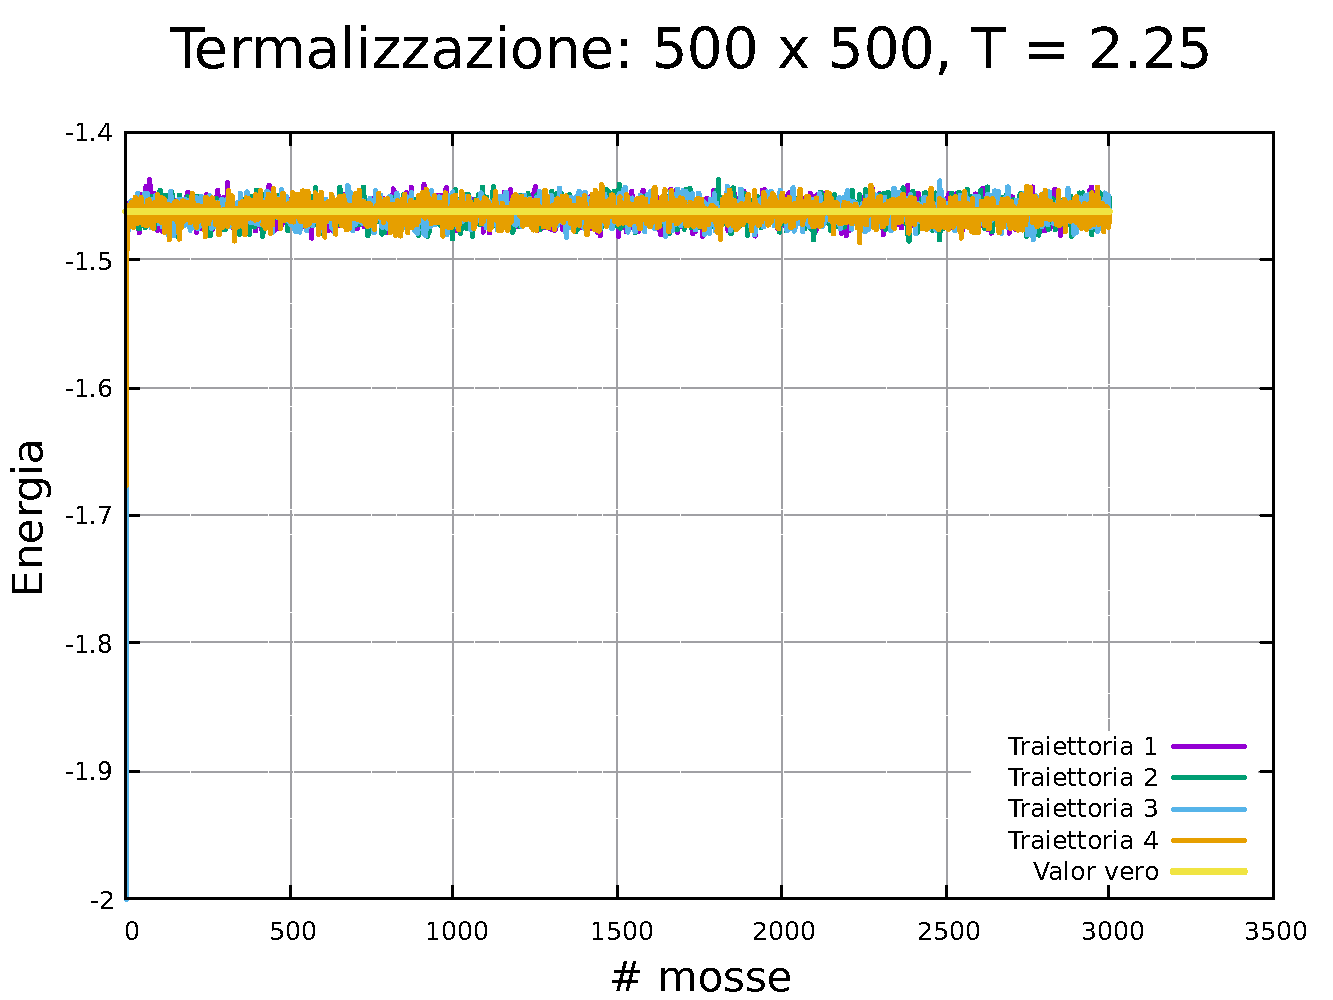
\includegraphics[width=\textwidth]{Immagini/simIsing2D/termW_500_2.25.pdf}
            
            \end{block}
        \end{column}
    
        \begin{column}{0.33\textwidth}
            \begin{block}{Auto-correlazione}

                \begin{itemize}[itemsep=0.5em, label=$\diamond$]
                    \item $t_{c}$ maggiori per $T \simeq T_c$
                    \item $t_{c}^{max}\,\simeq\,40$ sweeps
                \end{itemize}

                \vspace{0.5cm}

                \centering
                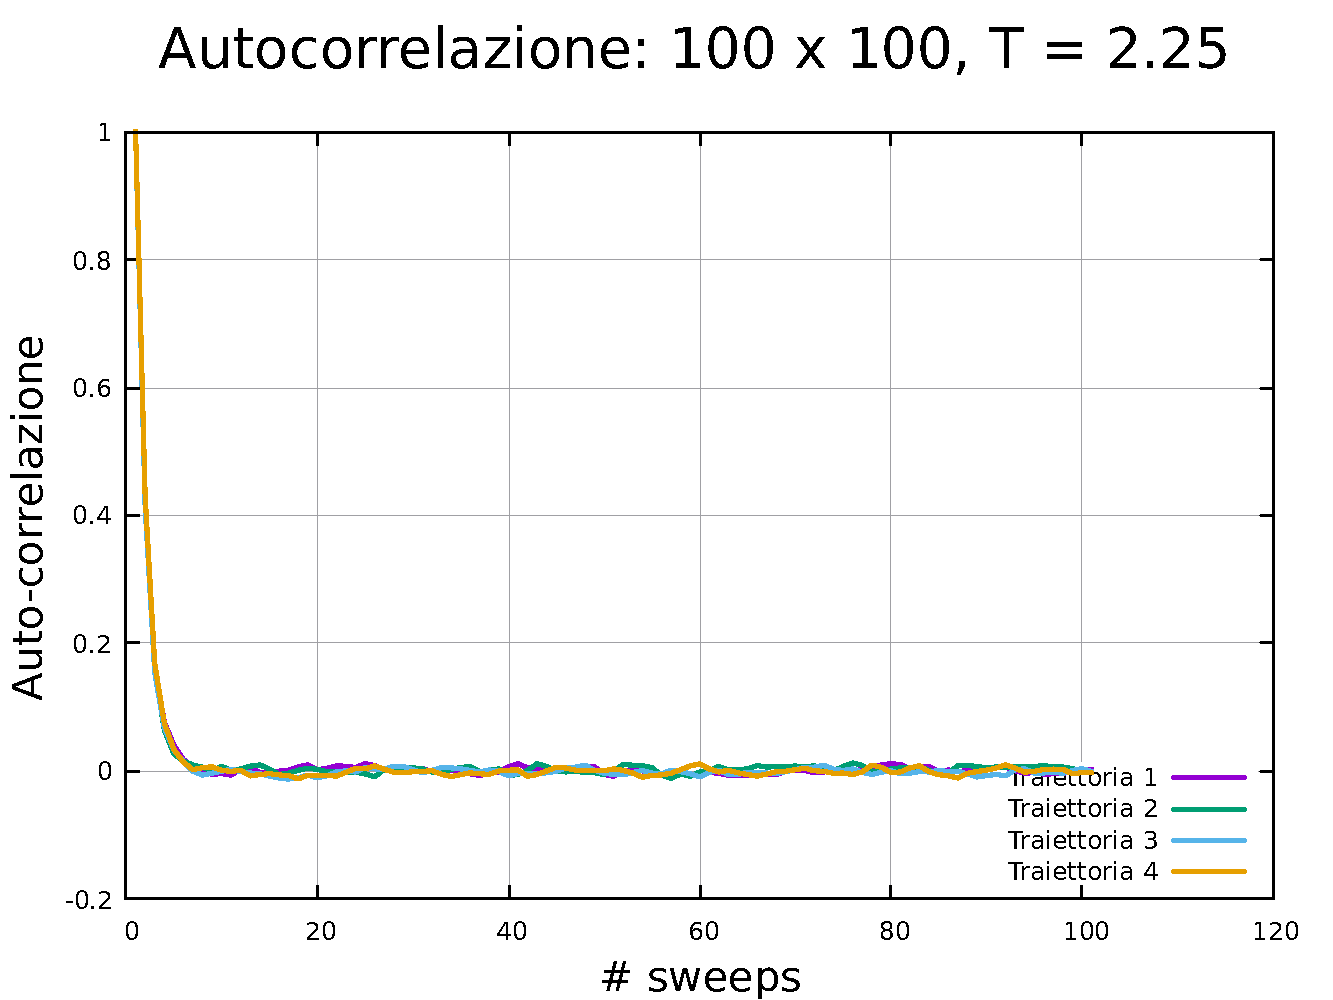
\includegraphics[width=\textwidth]{Immagini/simIsing2D/autoW_100_2.25.pdf}

            \end{block}
        \end{column}

        \begin{column}{0.33\textwidth}
            \begin{block}{Blocchi}
                
                \begin{itemize}[itemsep=0.5em, label=$\diamond$]
                    \item $l_{blk}$ maggiori per $T \simeq T_c$
                    \item $l_{blk}^{max}\,\simeq\,50$ sweeps
                \end{itemize}

                \vspace{0.5cm}

                \centering
                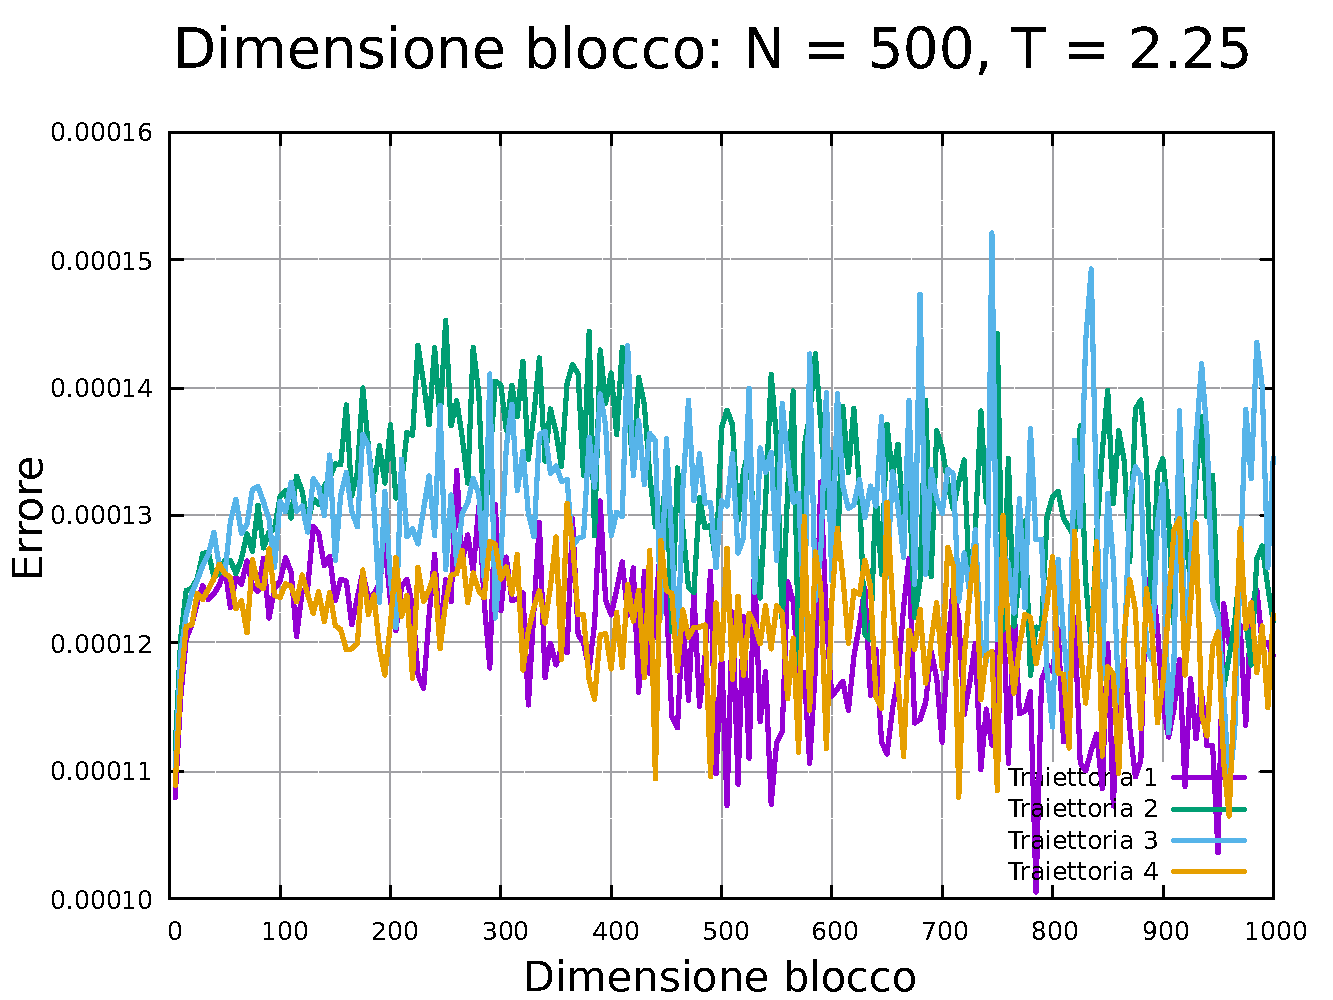
\includegraphics[width=\textwidth]{Immagini/simIsing2D/errW_500_2.25.pdf}

            \end{block}        
        \end{column}
    \end{columns}
\end{frame}



%-----------------------------------------%
%			  Terza slide				  %
%	   Studio della magnetizzazione   	  %
%-----------------------------------------%
\begin{frame}
    \frametitle{Magnetizzazione}
    \framesubtitle{}

    \begin{columns}
        \begin{column}{0.6\textwidth}

            \centering
            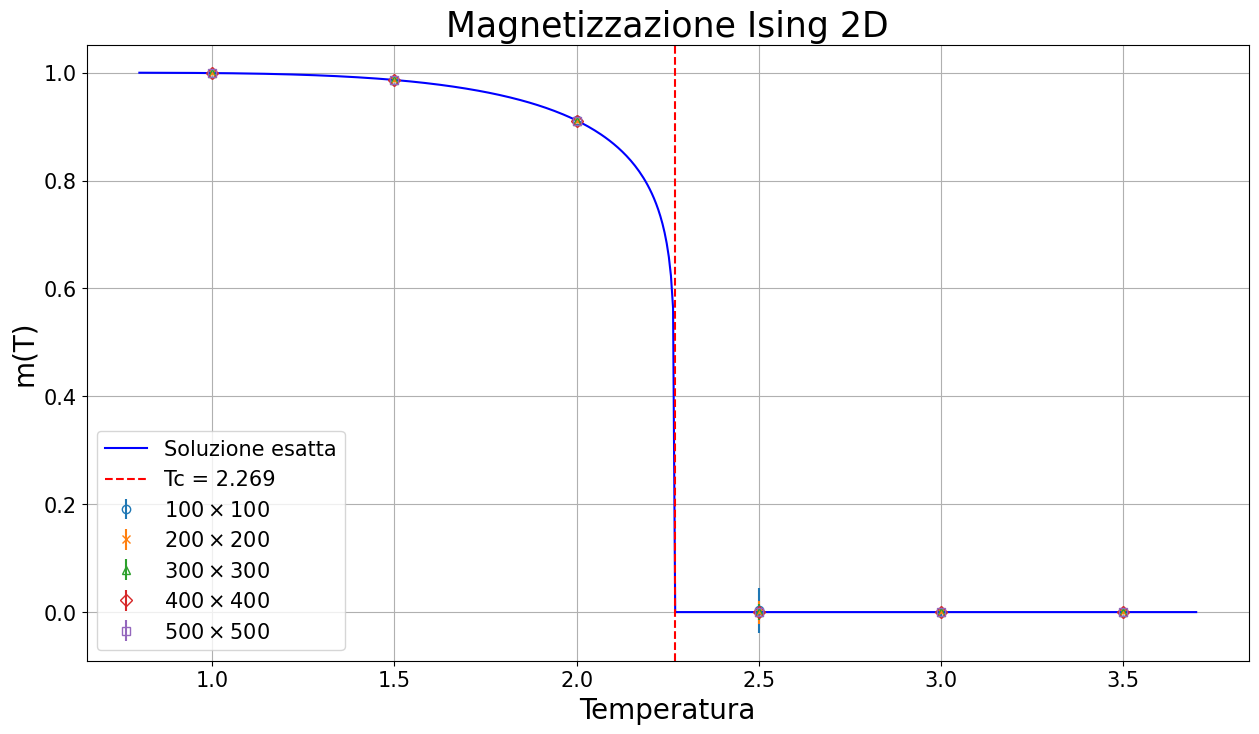
\includegraphics[width=\textwidth]{Immagini/simIsing2D/magn.png}

        \end{column}
    
        \begin{column}{0.4\textwidth}

                \begin{itemize}[itemsep=0.5em, label=$\diamond$]
                    \item Magnetizzazione spontanea per $T\,<\,T_c$
                    \item Transizione di fase a $T_c$
                \end{itemize}
            
        \end{column}
    \end{columns}

    \centering
    
\begin{tikzpicture}[thick, scale=1.2]
        \draw[->, line width=1mm] (0, 0) -- (10, 0);
        
        \node[below] at (0, 0) {Ferromagnetico};
        \node[below] at (10, 0) {Paramagnetico};
        
        \draw[fill=black] (5, 0) circle (2pt); 
        \node[above] at (5, 0) {$T_c$}; 
    \end{tikzpicture}

\end{frame}



%-----------------------------------------%
%			  Quarta slide				  %
%	   Studio dell'energia interna   	  %
%-----------------------------------------%
\begin{frame}
    \frametitle{Energia}
    \framesubtitle{}

    \begin{columns}
        \begin{column}{0.6\textwidth}

            \centering
            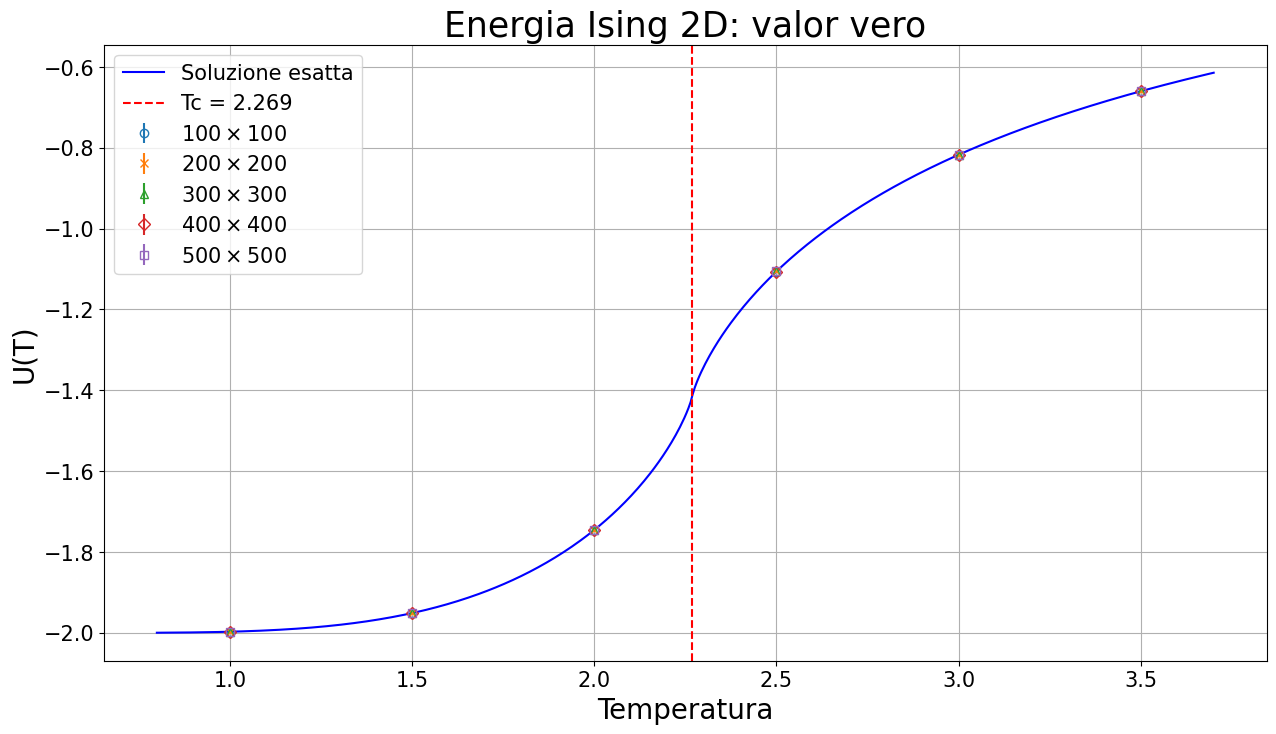
\includegraphics[width=\textwidth]{Immagini/simIsing2D/ene.png}

        \end{column}
    
        \begin{column}{0.4\textwidth}


                \begin{itemize}[itemsep=0.5em, label=$\diamond$]
                    \item copro tutto il reticolo con due legami per spin
                    \item picco del calore specifico a $T_c$
                \end{itemize}
            
        \end{column}
    \end{columns}

    \vspace{0.5cm}
    \centering
    $U\,=\,-NJ\coth{\left(2\beta J\right)}\left\{1\,+\,\frac{2}{\pi}\left[2\tanh^2\left(2\beta J\right)\,-\,1\right]\int_0^{\pi/2}\frac{d\phi}{\sqrt{1\,-\,k^2\sin^2{\left(\phi\right)}}}\right\}$

\end{frame}



%-----------------------------------------%
%		  	  Quinta slide - A			  %
%	      Studio della T critica    	  %
%-----------------------------------------%
\begin{frame}
    \frametitle{Dipendenza da $J$}
    \framesubtitle{}

    \begin{columns}
        \begin{column}{0.6\textwidth}

            \centering
            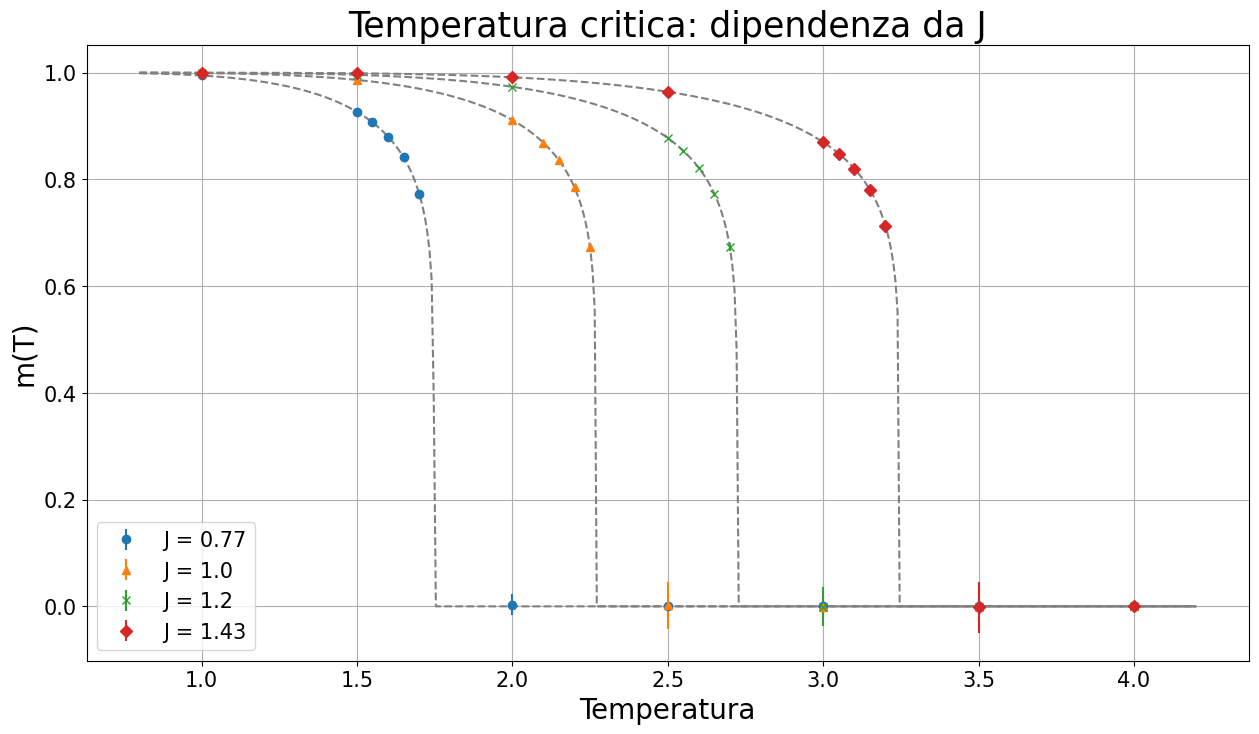
\includegraphics[width=\textwidth]{Immagini/simIsing2D/dipJ_Tc.png}

        \end{column}
    
        \begin{column}{0.4\textwidth}

                \begin{itemize}[itemsep=0.5em, label=$\diamond$]
                    \item Aumenta $J$, aumenta $T_c$
                    \item Presenza o meno di ordine dipende dall'intensità dell'interazione
                \end{itemize}
            
        \end{column}
    \end{columns}

\end{frame}



%-----------------------------------------%
%			Quinta slide - B			  %
%	   Studio del calore specifico   	  %
%-----------------------------------------%
\begin{frame}
    \frametitle{Regione critica}
    \framesubtitle{}

    \begin{columns}
        \begin{column}{0.5\textwidth}

            \centering
            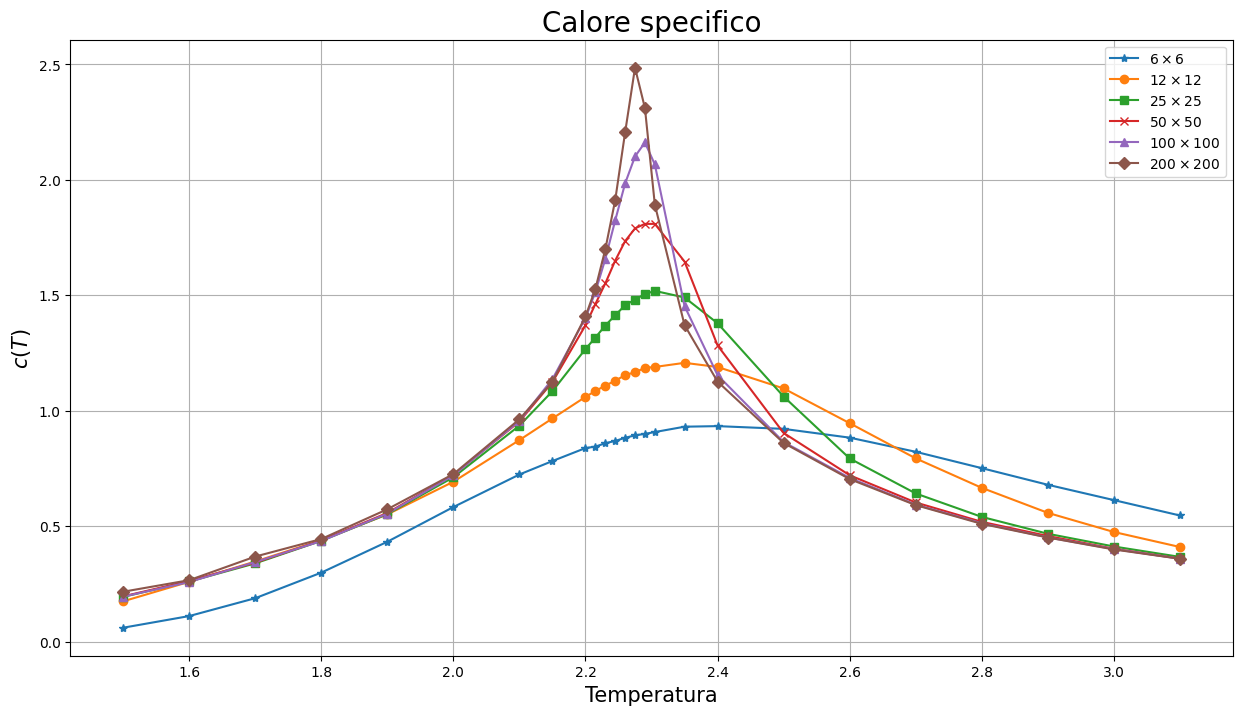
\includegraphics[width=\textwidth]{Immagini/simIsing2D/cp_zCrit.png}

        \end{column}
    
        \begin{column}{0.5\textwidth}
            
        \end{column}
    \end{columns}

\end{frame}



%-----------------------------------------%
%		   	  Settima slide				  %
%	     Studio con coarse graining   	  %
%-----------------------------------------%
\begin{frame}
    \frametitle{Coarse graining}
    \framesubtitle{}

    \centering
    \begin{tikzpicture}
        \node (img1) at (-1,0) {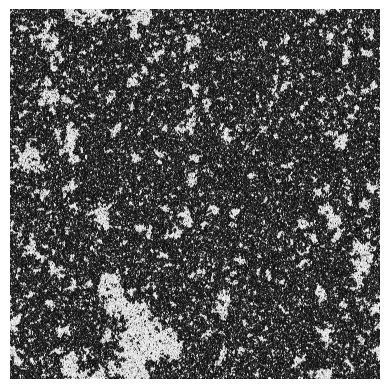
\includegraphics[width=0.4\textwidth]{Immagini/simIsing2D/cg_10000_Tc.png}};
        
        \node (img2) at (7,0) {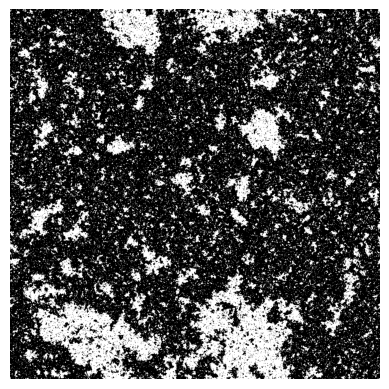
\includegraphics[width=0.4\textwidth]{Immagini/simIsing2D/cg_1000_Tc.png}};
        
        \draw[->,thick] (img1.east)  -- node[above] {CG} (img2.west);
    \end{tikzpicture}
    
\end{frame}



%-----------------------------------------%
%		   	   Ottava slide				  %
%	      Dimensione dei clusters   	  %
%-----------------------------------------%
\begin{frame}
    \frametitle{Dimensioni cluster}
    \framesubtitle{}

    \begin{columns}
        \begin{column}{0.6\textwidth}

            \centering
            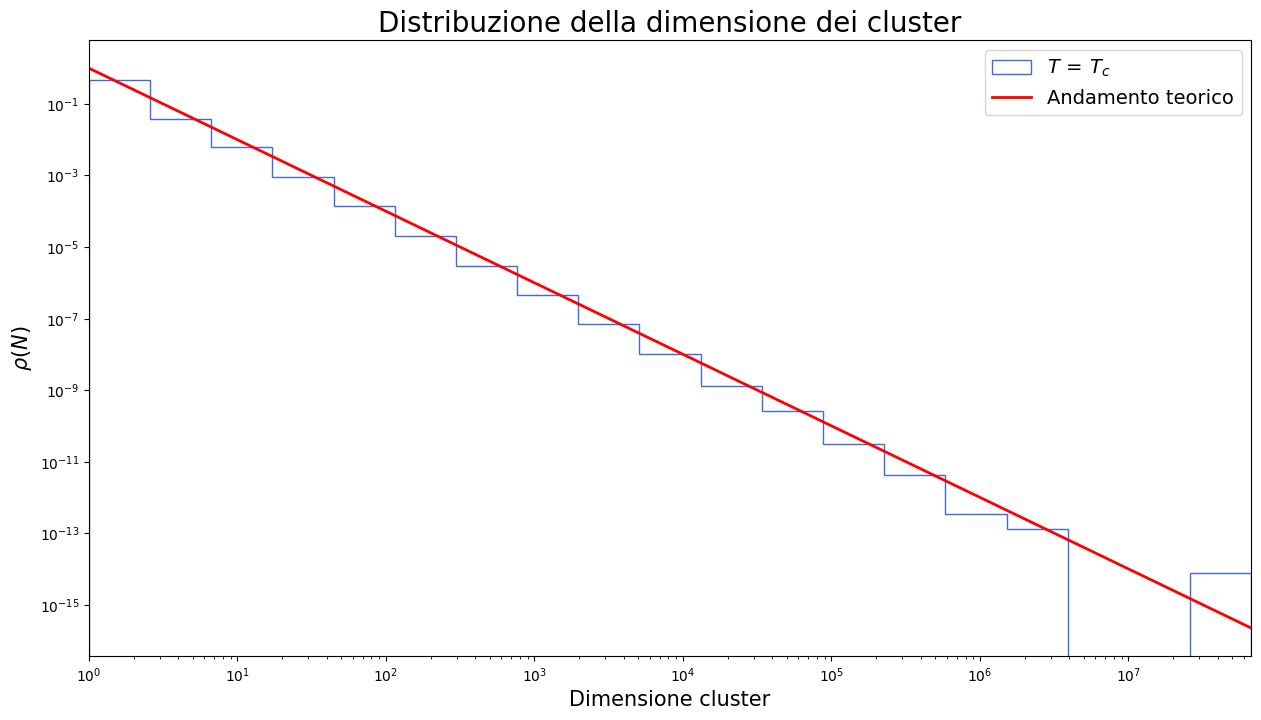
\includegraphics[width=\textwidth]{Immagini/simIsing2D/dimCl_Tc.png}

        \end{column}
    
        \begin{column}{0.4\textwidth}


                \begin{itemize}[itemsep=0.5em, label=$\diamond$]
                    \item $P\left(s\right) \propto s^{-\alpha}$
                    \item $\alpha \simeq 2$
                    \item perdita di un parametro di scala
                \end{itemize}
            
        \end{column}
    \end{columns}

    \centering
    
\begin{tikzpicture}[thick, scale=1.2]
        \draw[->, line width=1mm] (0, 0) -- (10, 0);
        
        \node[below] at (0, 0) {grandi cluster};
        \node[below] at (10, 0) {piccoli cluster};
        
        \draw[fill=black] (5, 0) circle (2pt); 
        \node[above] at (5, 0) {$T_c$}; 
    \end{tikzpicture}
    
\end{frame}
